%% Einleitung.tex
%% $Id: einleitung.tex 61 2012-05-03 13:58:03Z bless $
%%

\chapter{Einleitung}
\label{ch:Einleitung}
%% ==============================
Die Einleitung besteht aus der Motivation, der Problemstellung, der Zielsetzung und einem erster Überblick über den Aufbau der Arbeit.

%% ==============================
\section{Motivation}
%% ==============================
\label{ch:Einleitung:sec:Motivation}

\begin{itemize}
\item Definition
\item Wo findet das Knotenüberdeckungsproblem Anwendung?
\item Woher kommt die Komplexität?
\item Was macht eine schwere Instanz aus?
\item Wie sieht eine schwere Instanz aus?
\end{itemize}
Das \emph{Knotenüberdeckungsproblem}, oder englisch Vertex Cover, ist ein nachgewiesen NP-vollständiges Problem \cite{intract}. Um das Problem zu erklären, betrachten wir ein Netz von Haushalten, bei dem wir die Möglichkeit haben, in jedem Haushalt einen Stromgenerator zu platzieren, sodass durch alle mit diesem Haus verbundenen Leitungen Strom fließt. Ziel ist, ein stabiles Stromnetz zu schaffen, bei dem jede Leitung an mindestens eine Stromquelle angeschlossen ist. Nun ergibt sich das Problem, dass die Kosten für Stromgeneratoren erheblich sind und daher nur maximal \emph{k} Geräte angeschafft werden können. Es gilt also, aus den \emph{n} Häusern \emph{k} oder weniger auszuwählen, sodass jede Leitung von einem der Häuser in der Auswahl versorgt wird. 
\begin{figure}[htb]
\centering
  	{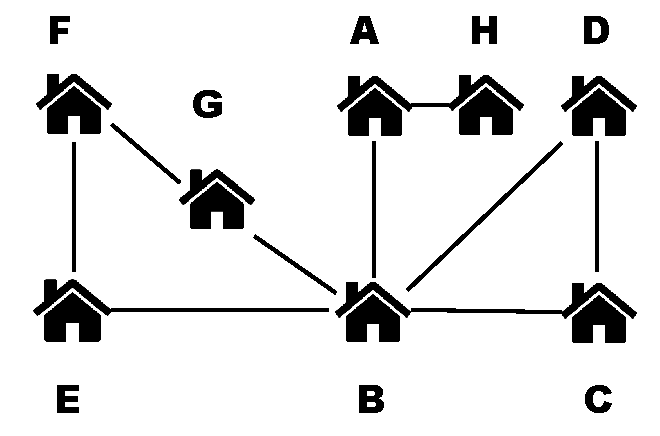
\includegraphics[width=.5\textwidth]{vertexcoverBsp.pdf}}
	\caption{Graph eines Stromnetzes \label{fig:vc}}
\centering
\end{figure}
In Abbildung \ref{fig:vc}\footnote{Icons in der Graphik von https://www.flaticon.com/}   sieht man ein Beispiel für eine solche Probleminstanz. Die Haushalte sind jeweils mit einem Buchstaben gekennzeichnet; jede Linie, beziehungsweise Kante eine Leitung zum Nachbarhaus. Hier ist es möglich eine Lösung für \emph{k} = 4 zu finden, also 4 Häuser mit Generatoren auszustatten, sodass alle Leitungen versorgt sind. Es ist leicht zu sehen, dass es keine Lösung mit weniger Häusern gibt. Um 4 Häuser, die das Problem lösen zu finden, betrachtet man nun jede Leitung und entscheidet, welches der beiden Häuser aufgenommen werden soll, da mindestens eins der beiden Häuser in der Lösungsmenge ist. Werden alle $2^{8}$ Möglichkeiten ausprobiert, finden sich die Lösung, dass wenn die Haushalte F, B, A und C oder F, B, A und D mit einem Generator ausgestattet werden, durch alle Leitungen Strom fließt. Für eine Problemgröße wie sie hier geschildert wird, bietet die \emph{Brute-Force}-Methode eine Lösung. Wenn nun allerdings ein Häusernetz mit mehreren Tausend Häusern und entsprechend vielen Leitungen zur Diskussion steht, ergibt sich so eine Menge an Möglichkeiten, die nicht in absehbarer Zeit verarbeitet werden kann. Für ein \emph{n} = 2000 bedeutet das $1.148 \cdot 10^{602}$ mögliche Kombinationen. Um die Explosion der Laufzeit zu verhindern 

%% ==============================
\section{Problemstellung}
%% ==============================
\label{ch:Einleitung:sec:Problemstellung}

\begin{itemize}
\item Effekt von Graphreduktionsalgorithmen auf die Problemkomplexität
\end{itemize}

%% ==============================
\section{Zielsetzung}
%% ==============================
\label{ch:Einleitung:sec:Zielsetzung}

\begin{itemize}
\item Kategorisierung der Regeln?
\item Bewertungskriterien für einen GRalgorithmus
	\begin{itemize}
	\item Laufzeit (Parametrisierung)
	\item Erwartete Reduktion/Wie oft wird die Regel angewandt
	\item Ressourcenverbrauch
	\item Wie gut ist das Ergebnis im Vergleich zu anderen Algorithmen?	
	\end{itemize}
\item Wie funktionieren die GRA in Kombination?
\item Wie sehen Graphen aus, auf die keine Regel anwendbar ist?
\item Wie sehen Graphen aus, auf die genau eine Regel anwendbar ist?
\item Welche Regeln werden untersucht?
\end{itemize}


%% ==============================
\section{Gliederung/Aufbau der Arbeit}
%% ==============================
\label{ch:Einleitung:sec:Gliederung}

Was enthalten die weiteren Kapitel? Wie ist die Arbeit aufgebaut? Welche Methodik wird verfolgt?


%%% Local Variables: 
%%% mode: latex
%%% TeX-master: "thesis"
%%% End: 
